\chapter{Edge detection}

\section{Illustrare i differenti tipi di edge presenti in un'immagine}
Nei punti di edge abbiamo un cambiamento brusco dell'intensità dei toni di grigio. L'edge è una proprietà associata ad un pixel calcolata dall'immagine in base al comportamento dei pixel nell'intorno del punto stesso. Un cambiamento della funzione immagine può essere descritto come un gradiente che punti in direzione della maggiore crescita della funzione immagine. Il gradiente avrà una sua magnitudo ed una sua direzione. La direzione dell'edge è perpendicolare rispetto la direzione del gradiente.

Possiamo identificare 4 tipi di edge, indicando nelle ordinate la magnitudo del gradiente e nelle ascisse una direzione x:
\begin{itemize}
	\item step: caratterizzato da un'improvvisa variazione del livello di grigio. E' rappresentato con una funzione a gradino
	\item roof: detto anche "doppia rampa", caratterizzato da una costante e graduale variazione fino a un	picco massimo dopo il quale si ritorna, in modo simmetrico, al valore di partenza
	\item line: il line, caratterizzato da un improvviso salto di livello di grigio al quale ne segue subito un altro verso il valore originario
	\item noisy: che è un edge a cui corrisponde una funzione della variazione dei livelli di grigio che parte da un valore e arriva a un altro, ma in modo irregolare
\end{itemize}

\begin{figure}[htbp]
	\centering
	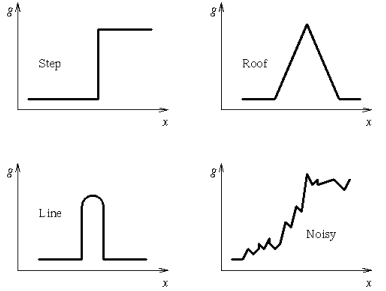
\includegraphics[scale=.5]{img/edge.png}
	\caption{Differenti tipi di edge}\label{fig:edge}
\end{figure}

\section{Classificazione degli edge detector}
L'edge detection è molto importante perché il successo del processing di più alto livello dipende molto da una buona rilevazione degli edge. Le immagini in scala di grigio contengono tantissime informazioni, molte delle quali sono irrilevanti. L'idea è quella di ridurre la mole di dati eliminando le informazioni di scarso interesse. Si cerca quindi di evidenziare quelli che poi saranno i contorni dell'immagine. Gli edge detector localizzano cambi improvvisi di intensità nella funzione
immagine.

Per localizzarli vi sono diversi modi e si possono suddividere in diverse classi:
\begin{itemize}
	\item Una prima classe è costituita da operatori di tipo gradiente che si basano su approssimazioni della derivata prima
	
	\item La seconda classe è costituita da operatori che trattano l'immagine come una superficie vista come approssimazione discreta di una funzione bidimensionale continua, di cui si fa la derivata prima (in tal caso gli edge sono i punti in cui la derivata assume valori elevati) o la	derivata seconda (gli edge sono i punti in cui la derivata attraversa lo zero)
	
	\item La terza classe di operatori cerca di risolvere il problema del rumore che può influenzare la bontà dell'edge detector. Viene inizialmente applicato un filtro (per esempio il filtro gaussiano) all'immagine su cui successivamente viene applicato un operatore differenziale
\end{itemize} 


\subsection{Dettagli?}
Essi si basano sulle derivate parziali locali della funzione immagine. Le derivate sono maggiori nei punti in cui la funzione subisce un rapido cambiamento (sono i punti di edge). L'operatore gradiente ha il compito di indicare una tali punti aumentandone il dettaglio. Sfortunatamente applicando un operatore gradiente su un immagine il livello di rumore cresce notevolmente.
Gli operatori basati su gradiente possono essere divisi in tre categorie:
\begin{enumerate}
	\item operatori	che approssimano le	derivate tramite differenze (Roberts, Laplace, Prewitt, Sobel, Robinson, Kirsch)
	\begin{enumerate}
		\item invarianti alla rotazione (come il Laplaciano) richiedono una sola maschera di convoluzione
		\item per approssimare la derivata prima servono diverse maschere di convoluzione e	l'orientazione viene stimata sulla base del miglior matching tra diversi semplici pattern
	\end{enumerate}
	
	\item operatori basati sullo zero crossing della derivata seconda
	\begin{enumerate}
		\item Marr-Hildreth
		\item Canny Edge Detector
	\end{enumerate}
	
	\item operatori che confrontano l'immagine con modelli parametrici di edge
	\begin{itemize}
		\item i modelli parametrici descrivono molto dettagliatamente gli edge (più di norma e \v{o}direzione) ma sono computazionalmente più costosi
	\end{itemize}
\end{enumerate}

Una categoria degli operatori basati su gradiente approssimano le derivate prime tramite differenze. Gli operatori gradiente che esaminano un piccolo intorno del punto sono di fatto delle convoluzioni e possono pertanto essere espressi per mezzo di maschere. Gli operatori che sono in grado di rilevare gli edge sono rappresentati da una serie di maschere, ognuna corrispondente ad una certa direzione.

\section{Illustrare i metodi per l’edge detection basati sull’approssimazione delle derivate prime}
Gli operatori che si basano sull'utilizzo della derivata prima (nella sua approssimazione nel caso discreto) consistono nell'applicazione di filtri, attraverso delle maschere di convoluzione. Ogni specifico operatore ha le sue maschere di convoluzione, solitamente per due o più diverse direzioni del gradiente.
\begin{itemize}
	\item L'operatore di Roberts è quello computazionalmente più efficiente (utilizza una maschera 2x2) però va a evidenziare anche punti che non sono di edge, essendo molto influenzato dal rumore presente nell'immagine.
	
	\item Gli operatori di tipo compass consentono di individuare non solo il valore del gradiente ma anche l'orientazione degli edge, perché utilizzano delle maschere diverse per ogni tipo di orientazione. A ogni punto vengono applicate tutte le maschere, dopodiché per capire qual è la direzione dell'edge basta vedere quale maschera ha fornito la risposta massima. La risposta totale del gradiente è o la somma o il massimo delle risposte delle singole matrici.
\end{itemize}

\section{Descrivere la tecnica della non-maxima suppression}
La non-maxima suppression è una tecnica di edge detection utilizzata per identificare i pixel di edge partendo dalla mappa del gradiente. I pixel considerati di edge sono quelli che hanno un valore di gradiente superiore ai due pixel che lo precedono e che lo seguono, nella direzione del gradiente.

\section{Illustrare il Marr-Hildreth edge detector}
L'operatore Marr-Hildreth (detto anche LoG) è un operatore di edge detection che unisce gli operatori gaussiano e laplaciano. La sua applicazione si compone di tre passi fondamentali:
\begin{itemize}
	\item applicazione del filtro di smoothing gaussiano così da attenuare il rumore presente nell'immagine
	
	\item applicazione dell'operatore laplaciano che calcola la derivata seconda dell'immagine evidenziando i punti in cui subisce brusche variazioni
	
	\item localizzazione dei punti in cui la derivata seconda attraversa lo zero (zero crossing)
\end{itemize}

In realtà, grazie alla linearità delle operazioni, viene applicato il laplaciano sulla matrice di convoluzione dell'operatore gaussiano, che viene poi applicata all'immagine.

\section{Illustrare il Canny edge detector}
Il Canny Edge Detector è ottimo edge detector per il white noise. È riconosciuto come l'operatore migliore per l'edge detection per tre motivi:
\begin{enumerate}
	\item Ricerca: gli edge importanti vengono sempre rilevati
	\item Localizzazione: la distanza tra il punto in cui l'edge viene rilevato e la sua locazione reale è minimale
	\item Le risposte multiple (più localizzazioni per un singolo edge) sono ridotte al minimo (questo punto ricopre in parte ciò che viene definito nel primo punto)
\end{enumerate}

\subsection{Implementazione}
\begin{itemize}
	\item Si applica un filtro Gaussiano all'immagine
	
	\item Si calcola il gradiente (norma e direzione) mediante la tecnica delle differenze: a questo scopo vengono utilizzate due maschere di convoluzione 2x2 che restituiscono rispettivamente $p(x,y)$ e $q(x,y)$ dell'edge secondo la formula:
	
	\item Si applica la soppressione dei non-maxima alla norma del gradiente in modo da assottigliare
	gli edge che altrimenti sarebbero troppo spessi
	
	
	\item Si applica la soppressione dei non-maxima alla norma del gradiente in modo da assottigliare gli edge che altrimenti sarebbero troppo spessi
	
	\item Si usa una doppia sogliatura per trovare e collegare gli edge: si definiscono due soglie $\tau_1$ e $\tau_2$ tali che $\tau_2 \approx 2 \tau_1$ e si producono due mappe degli edge $T_1(x,y)$ e $T_2(x,y)$. La mappa costruita con la soglia più alta conterrà sicuramente pochissimi edge falsi ma quelli veri risulteranno probabilmente spezzati per cui la mappa finale viene costruita partendo da $T_2(x,y)$ e collegando i contorni solo se, posizionatisi all'estremo di un edge, nell'8-intorno associato a	tale punto in $T_1(x,y)$ ci sono degli edge che possono essere collegati. L'algoritmo continua a collegare edge sino a quando è stato colmato il percorso vuoto che conduce ad un altro edge in $T_2(x,y)$
\end{itemize}

\section{Quali sono i vantaggi e gli svantaggi degli edge detector?}
Gli edge detector in generale sono fondamentali per poter proseguire ai livelli superiori
dell'elaborazione di un'immagine (come la segmentazione). Per descrivere vantaggi e svantaggi degli edge detector è opportuno dividere gli operatori in classi.
\begin{enumerate}
	\item La \textbf{prima classe} contiene operatori gradiente di dimensione 3x3 o 5x5 (Prewitt, Robert, Sobel, Laplacian). Questi operatori lavorano abbastanza bene su scene sintetiche ma disegnano degli edge	molto spessi, per cui spesso necessitano di un operazione di thinning successiva. L'operatore di Roberts ha un'alta sensibilità al rumore a causa del basso numero di pixel usati per calcolare il gradiente. Uno svantaggio dell'operatore laplaciano è che può rispondere in modo doppio a certi edge a causa del rumore.Gli operatori che si basano sul calcolo della derivata prima (Prewitt, Robert, Sobel, Kirsch, Robinson) forniscono, oltre al suo modulo, anche la direzione dell'edge.
	
	\item Nella \textbf{seconda classe} sono contenuti gli operatori che si basano sul concetto di zero crossing. Ovvero individuando l'intorno in cui si presenta l'attraversamento dello zero nelle differenze fra le derivate seconde. Fanno parte di questo gruppo il LoG e il Canny edge detector. I LoG ha il vantaggio, rispetto agli operatori della prima classe, di ridurre il rumore in fase di preprocessing e	quindi non fornisce risposte doppie agli per gli edge.
	
	Il Canny edge detector è l'ideale per edge di tipo step corrotte da white noise. La sua ottimalità è dovuta al rispetto di 3 criteri fondamentali:
	\begin{itemize}
		\item Trova tutti gli edge importanti
		
		\item La distanza tra la posizione reale dell'edge e l'edge individuato è minima
		
		\item Minimizza le risposte multiple perché effettua la soppressione degli edge che non hanno il gradiente massimo
	\end{itemize}
\end{enumerate}

\section{Quali sono i criteri per valutare la bontà di un edge detector?}
I criteri per valutare la bontà di un edge detector sono:
\begin{itemize}
	\item la probabilità che vengano classificati come edge degli edge falsi
	
	\item la probabilità che non vengano riportati degli edge significativi
	
	\item l'errore commesso nella valutazione degli angoli fra gli edge
	
	\item la distanza tra gli edge estratti e gli edge reali, cioè quanto effettivamente gli edge estratti corrispondono agli edge reali
	
	\item la tolleranza agli angoli, alle giunzioni, ai punti che rappresentano degli spigoli, cioè quanto l'operatore riesce a localizzarli bene
\end{itemize}

La bontà di un edge detector, e quindi l'insieme di questi requisiti, viene valutata mediante un parametro F \footnote{vedi slide 13 lect09 new}. Il risultato è sempre compreso fra 0 e 1. Un valore corrispondente a 1 indica che l'edge detector estrae esattamente tutti gli edge significativi. La bontà di un edge detector si valuta quindi facendolo lavorare su un'immagine teorica e aggiungendo del rumore per vedere se il parametro F rimane vicino a 1.